% Template for Cogsci submission with R Markdown

% Stuff changed from original Markdown PLOS Template
\documentclass[10pt, letterpaper, hidelinks]{article}

\usepackage{cogsci}
\usepackage{pslatex}
\usepackage{float}
\usepackage{caption}

% amsmath package, useful for mathematical formulas
\usepackage{amsmath}

% amssymb package, useful for mathematical symbols
\usepackage{amssymb}

% hyperref package, useful for hyperlinks
\usepackage{hyperref}

% graphicx package, useful for including eps and pdf graphics
% include graphics with the command \includegraphics
\usepackage{graphicx}

% Sweave(-like)
\usepackage{fancyvrb}
\DefineVerbatimEnvironment{Sinput}{Verbatim}{fontshape=sl}
\DefineVerbatimEnvironment{Soutput}{Verbatim}{}
\DefineVerbatimEnvironment{Scode}{Verbatim}{fontshape=sl}
\newenvironment{Schunk}{}{}
\DefineVerbatimEnvironment{Code}{Verbatim}{}
\DefineVerbatimEnvironment{CodeInput}{Verbatim}{fontshape=sl}
\DefineVerbatimEnvironment{CodeOutput}{Verbatim}{}
\newenvironment{CodeChunk}{}{}

% cite package, to clean up citations in the main text. Do not remove.
\usepackage{apacite}

% KM added 1/4/18 to allow control of blind submission
\cogscifinalcopy

\usepackage{color}

% Use doublespacing - comment out for single spacing
%\usepackage{setspace}
%\doublespacing


% % Text layout
% \topmargin 0.0cm
% \oddsidemargin 0.5cm
% \evensidemargin 0.5cm
% \textwidth 16cm
% \textheight 21cm

\title{Frequency-dependent preference extremity arises from a
noisy-channel processing model}

\usepackage{environ}
\usepackage[section]{placeins}

\author{{\large \bf Zachary Houghton (znhoughton@ucdavis.edu)} \\ Department of Linguistics, 1 Shields Avenue \\ Davis, CA 95616 USA \AND {\large \bf Emily Morgan (eimorgan@ucdavis.edu)} \\ Department of Linguistics, 1 Shields Avenue \\ Davis, CA 95616 USA}

\newlength{\cslhangindent}
\setlength{\cslhangindent}{1.5em}
\newenvironment{CSLReferences}%
  {}%
  {\par}

\begin{document}

\maketitle

\begin{abstract}
Language often has different ways to express the same or similar
meanings. Despite this, however, people seem to have preferences for
some ways over others. For example, people overwhelmingly prefer
\emph{bread and butter} to \emph{butter and bread}. Previous research
has demonstrated that these ordering preferences grow stronger with
frequency (i.e., frequency-dependent preference extremity). In this
paper we demonstrate that this frequency-dependent preference extremity
can be accounted for by noisy-channel processing models (e.g., Gibson et
al., 2013; Levy, 2008). We also show that this preference extremity can
only be accounted for if the listener infers more noise than the speaker
produces. Finally, we show that the model can account for the
language-wide distribution of binomial ordering preferences.

\textbf{Keywords:}
Frequency-dependent preference extremity; Noisy-channel processing;
Psycholinguistics.
\end{abstract}

\NewEnviron{myequation}{%
\begin{equation}
\scalebox{1}{$\BODY$}
\end{equation}
}

\hypertarget{introduction}{%
\section{Introduction}\label{introduction}}

Speakers are often confronted with many different ways to express the
same meaning. A customer might ask whether a store sells ``radios and
televisions'', but they could have just as naturally asked whether the
store sells ``televisions and radios.'' However, despite conveying the
same meaning, speakers sometimes have strong preferences for one choice
over competing choices (e.g., preference for \emph{men and women} over
\emph{women and men}, Benor \& Levy, 2006; Morgan \& Levy, 2016a). These
preferences are driven to some extent by generative preferences (e.g.,
preference for short words before long words), however they are
sometimes violated by idiosyncratic preferences (e.g., \emph{ladies and
gentlemen} preferred despite a general men-before-women generative
preference, Morgan \& Levy, 2016b).

Interestingly, ordering preferences for certain constructions, such as
binomial expressions, are often more extreme for higher frequency items
(e.g., \emph{bread and butter}). That is, higher-frequency items
typically have more polarized preferences (Liu \& Morgan, 2020, 2021;
Morgan \& Levy, 2015, 2016b, 2016a). This phenomenon is called
\emph{frequency-dependent preference extremity}, and while there is
evidence of it in several different constructions, it is still unclear
what processes this phenomenon is driven by. For example, it could be a
consequence of learning processes or a consequence of sentence
processing more broadly. In the present paper we examine whether a
noisy-channel processing model (Gibson et al., 2013) combined with
transmission across generations (Kirby et al., 2008; Reali \& Griffiths,
2009) can account for frequency-dependent preference extremity.

\hypertarget{frequency-dependent-preference-extremity}{%
\subsection{Frequency-dependent preference
extremity}\label{frequency-dependent-preference-extremity}}

Frequency-dependent preference extremity has been documented for a
variety of different constructions in English (Liu \& Morgan, 2020,
2021; Morgan \& Levy, 2015, 2016b). For example, Morgan \& Levy (2015)
demonstrated that more frequent binomial expressions (e.g., \emph{bread
and butter}) are more polarized (i.e., are preferred in one order
overwhelmingly more than the alternative). These ordering preferences
are also not simply a result of generative ordering preferences (e.g.,
short words before long words, Morgan \& Levy, 2016a). Interestingly,
Morgan \& Levy (2016b) even showed that the distribution of binomial
orderings at the corpus-wide level are different than what would be
expected given the generative preferences for the binomials (see Figure
\ref{fig:corpusplot1}).

Additionally, Liu \& Morgan (2020) demonstrated that the dative
alternation in English also shows evidence of frequency-dependent
preference extremity (e.g., \emph{give} \emph{the ball to him}~vs
\emph{give him the ball}). Specifically, they demonstrated that higher
frequency verbs have more polarized preferences with respect to the
dative alternation. Similarly, Liu \& Morgan (2021) showed that in
adjective-adjective-noun constructions, the adjective orderings also
show frequency-dependent preference extremity. That is, adjectives in
adjective-adjective-noun constructions with higher overall frequencies
(i.e., the summed counts of both orderings) show stronger ordering
preferences, even after taking into account generative preferences of
adjective orderings.

Interestingly, frequency-dependent preference extremity patterns
differently from rule-following regularization processes (e.g.,
morphological regularization) where it is the low-frequency items that
become more regular (rather than the high-frequency items, e.g.
Singleton \& Newport, 2004). For example, Schneider et al. (2020)
demonstrated through a noisy-channel processing model that
regularization can arise from learners attributing variation in the
low-frequency items to noise. On the other hand, frequency-dependent
preference extremity patterns more similarly to other processes, such as
semantic entrenchment, where it is the high-frequency items that develop
strict preferences (Harmon \& Kapatsinski, 2017; Theakston, 2004). For
example, people are generally more willing to accept a low-frequency
intransitive verb in a transitive context than a high-frequency
intransitive verb (e.g., \emph{He vanished it} is judged to be more
acceptable than \emph{He disappeared it}, Kapatsinski, 2018; Robenalt \&
Goldberg, 2015; Theakston, 2004).

Why is it that it is the high-frequency items that develop more
polarized preferences in frequency-dependent preference extremity? One
possibility is that it occurs as an interaction between imperfect
learning and transmission across generations. For example, it's possible
that while learners of a language are in general very good at learning
the statistical patterns in the language (e.g., Saffran et al., 1996; Yu
\& Smith, 2007), they may do so imperfectly and with a bias towards
preference extremity. For example, if a learner hears 70 tokens of
\emph{bread and butter} and 30 tokens of \emph{butter and bread}, they
may imperfectly infer the ordering preference and transmit the language
with a more skewed distribution (e.g., 75 tokens \emph{bread and butter}
and 25 tokens of \emph{butter and bread}). Indeed, previous studies have
shown that learners will reproduce the more frequent item at an even
higher rate than they heard it (Harmon \& Kapatsinski, 2017; Hudson Kam
\& Newport, 2009). As the language is transmitted from generation to
generation, it is possible this compounds until the highest-frequency
items develop polarized ordering preferences.

Following this logic, Morgan \& Levy (2016b) investigated whether
frequency-dependent preference extremity can arise as a result of
imperfect learning across generations. They found that a data generation
model with a frequency-\emph{independent} bias can result in
frequency-\emph{dependent} preference extremity across generations of
learners in a 2-alternative iterated learning paradigm. They argued that
frequency-dependent preference extremity emerges because for
low-frequency items, the preference extremity bias cannot overcome the
learner's generative preferences for maintaining variation, but for
high-frequency items, it can. In other words, for lower frequency items,
learners may rely more on their generative preferences because they
haven't heard the item very much. As the language is transmitted across
many generations, it may result in frequency-dependent preference
extremity.

While there is good evidence that a frequency-\emph{independent}
preference extremity bias can account for frequency-dependent preference
extremity across generations, it remains unclear what processes in
language transmission are analogous to this preference extremity bias.

\hypertarget{noisy-channel-processing}{%
\subsection{Noisy-channel Processing}\label{noisy-channel-processing}}

One possibility is that the frequency-independent preference extremity
bias is a product of noisy-channel processing (Gibson et al., 2013).
Listeners are confronted with a great deal of noise in the form of
perception errors (e.g., a noisy environment) and even production errors
(speakers don't always say what they intended to, Gibson et al., 2013).
In order to overcome these errors, a processing system must take into
account the noise of the system, for example by probabilistically
determining whether the perceived utterance was infact intended by the
speaker.

Indeed, there is evidence that our processing system does take noise
into account. For example, Ganong (1980) found that people will process
a non-word as being a word under noisy conditions. Additionally, Albert
Felty et al. (2013) demonstrated that when listeners do misperceive a
word, the word that they believe to have heard tends to be higher
frequency than the target word. Further, Keshev \& Meltzer-Asscher
(2021) found that in Arabic, readers will even process ambiguous
subject/object relative clauses as the more frequent interpretation,
even if this interpretation compromises subject-verb agreement. These
results taken together suggest that misperceptions may sometimes
actually be a consequence of noisy-channel processing (although it's
worth noting that good-enough processing theories also make very similar
predictions, e.g., Ferreira \& Patson, 2007).

Further, people will even process \emph{grammatical} utterances, as a
more frequent or plausible interpretation (Christianson et al., 2001;
Levy, 2008; Poppels \& Levy, 2016). This can even arise in two
interpretations that cannot both be consistent with the original
sentence. For example, Christianson et al. (2001) demonstrated that when
people read the sentence \emph{While the man hunted the deer ran into
the woods}, people will answer in the affirmative for both \emph{Did the
man hunt the deer?} and \emph{Did the dear run into the woods?}. Levy
(2008) argued that this phenonenon was explained by noisy-channel
processing, since a single insertion results in plausible, grammatical
constructions for both meanings (\emph{While the man hunted it the deer
ran into the woods} vs \emph{While the man hunted the deer it ran into
the woods}).

In order to account for findings like these, Gibson et al. (2013)
developed a computational model that demonstrated how a system might
take into account noise (see Levy, 2008 for a similar approach).
Specifically, their model operationalizes noisy-channel processing as a
Bayesian process where a listener estimates the probability of the
speaker's intended utterance given what they perceived. Specifically,
this is operationlized as being proportional to the prior probability of
the intended utterance multiplied by the probability of the intended
utterance being corrupted to the perceived utterance (See Equation
\ref{eq:gibsonnoisy}):

\begin{equation}
\label{eq:gibsonnoisy}
P(S_i|S_p) \propto P(S_i) P(S_i \to S_p)
\end{equation}

\noindent where \(P(S_i|S_p)\) is the probability of the intended
utterance given the perceived utterance, \(P(S_i)\) is the prior
probability of the intended utterance, and \(P(S_i \to S_p)\) is the
probability of the perceived utterance (\(S_p\)) given the intended
utterance (\(S_i\)). If the perceived utterance is \emph{butter and
bread}, for example, the listener can infer the probability that the
intended utterance was \emph{bread and butter} or \emph{butter and
bread}.

Gibson et al. (2013)'s model made a variety of interesting predictions.
For example, the model predicted that when people are presented with an
implausible sentence (e.g., \emph{the mother gave the candle the
daughter}), they should be more likely to interpret the plausible
version of the sentence (e.g., \emph{the mother gave the candle to the
daughter}) if there is increased noise (e.g., by adding syntactic errors
to the filler items, such as a deleted function word). Their model also
predicted that increasing the likelihood of implausible events (e.g., by
adding more filler items that were implausible, such as \emph{the girl
was kicked by the ball}) should increase the rate of implausible
interpretations of the sentence. Interestingly both of these results
were born out in their experimental data. In a follow up study, Poppels
\& Levy (2016) further demonstrated that word-exchanges (e.g., \emph{The
ball kicked the girl} vs \emph{The girl kicked the ball}) are also taken
into account by comprehenders. These results taken together suggest that
humans do utilize a noisy-channel system in processing.

In addition to Gibson et al. (2013), previous research has demonstrated
that noisy-channel processing models may also account for certain types
of regularization (e.g., Ferdinand et al., 2019; Schneider et al.,
2020). For example, as mentioned earlier, Schneider et al. (2020) has
demonstrated that a noisy-channel model can account for some
rule-following regularization processes (e.g., morphological
regularization). However, it is unclear whether noisy-channel processing
models can also account for frequency-dependent preference extremity.

\hypertarget{present-study}{%
\subsection{Present Study}\label{present-study}}

Given the evidence of noisy-channel processing, it is possible that the
frequency-dependent preference extremity that Morgan \& Levy (2016b) saw
is a product of listeners' noisy-channel processing. Perhaps when
learners hear the phrase \emph{butter and bread}, they think the speaker
intended \emph{bread and butter}, which results in an activation of
\emph{bread and butter} even though they didn't hear it. This activation
could potentially even be stronger for \emph{bread and butter} than
\emph{butter and bread} in cases where the listener thinks the speaker
made a mistake. Further, this may compound over time for high frequency
items, but not for low frequency items. Thus, the present study examines
whether Gibson et al. (2013)'s noisy-channel processing model can also
predict frequency-dependent preference extremity across generations of
language transmission.

\hypertarget{dataset}{%
\section{Dataset}\label{dataset}}

Following Morgan \& Levy (2016b), we use Morgan \& Levy (2015)'s corpus
of 594 Noun-Noun binomial expressions (e.g., \emph{bread and butter}).
There is evidence that human binomial ordering preferences are driven by
a combination of generative preferences and observed preferences.
Generative preferences are abstract constraints on ordering preferences,
such as a preference for short words before long words, or male-coded
terms before female-coded terms. The observed preference for a given
binomial is the percentage that a given binomial occurs in alphabetical
vs nonalphabetical form. That is, if \emph{cats and dogs} appears 40
times in a corpus, and \emph{dogs and cats} appears 60 times, then the
observed preference for the alphabetical form is 0.4. The corpus also
contains the overall frequency (total count of alphabetical and
nonalphabetical forms for a given binomial) which has been shown to
affect the strength of ordering preferences (Morgan \& Levy, 2016b). A
detailed description of the constraints is listed below:

\begin{enumerate}
\def\labelenumi{\arabic{enumi}.}
\item
  The estimated generative preferences for each binomial, which are
  values between 0 and 1 representing the alphabetical ordering
  preferences (a neutral reference order), estimated from various
  phonological and semantic features that are known to influence
  binomial ordering preferences (Morgan \& Levy, 2015). The generative
  constraints are calculated using Morgan \& Levy (2015)'s model. Values
  closer to zero represent a generative preference for the
  nonalphabetical order, while values closer to 1 represent a generative
  preference for the alphabetical order.
\item
  The observed binomial orderings preferences (hereafter: observed
  preferences) which are the proportion of binomial orderings that are
  in alphabetical order for a given binomial. A visualization of the
  distribution of observed preferences and generative preferences is
  included below in Figure \ref{fig:corpusplot1}.
\item
  The overall frequency of a binomial expression (the frequency of AandB
  plus the frequency of BandA). Frequencies were obtained from the
  Google Books \emph{n}-grams corpus (Lin et al., 2012), which is orders
  of magnitude larger than the language experience of an individual
  speaker, and thus provides reliable frequency estimates for these
  expressions.
\end{enumerate}

\begin{CodeChunk}
\begin{figure}[tb]

{\centering 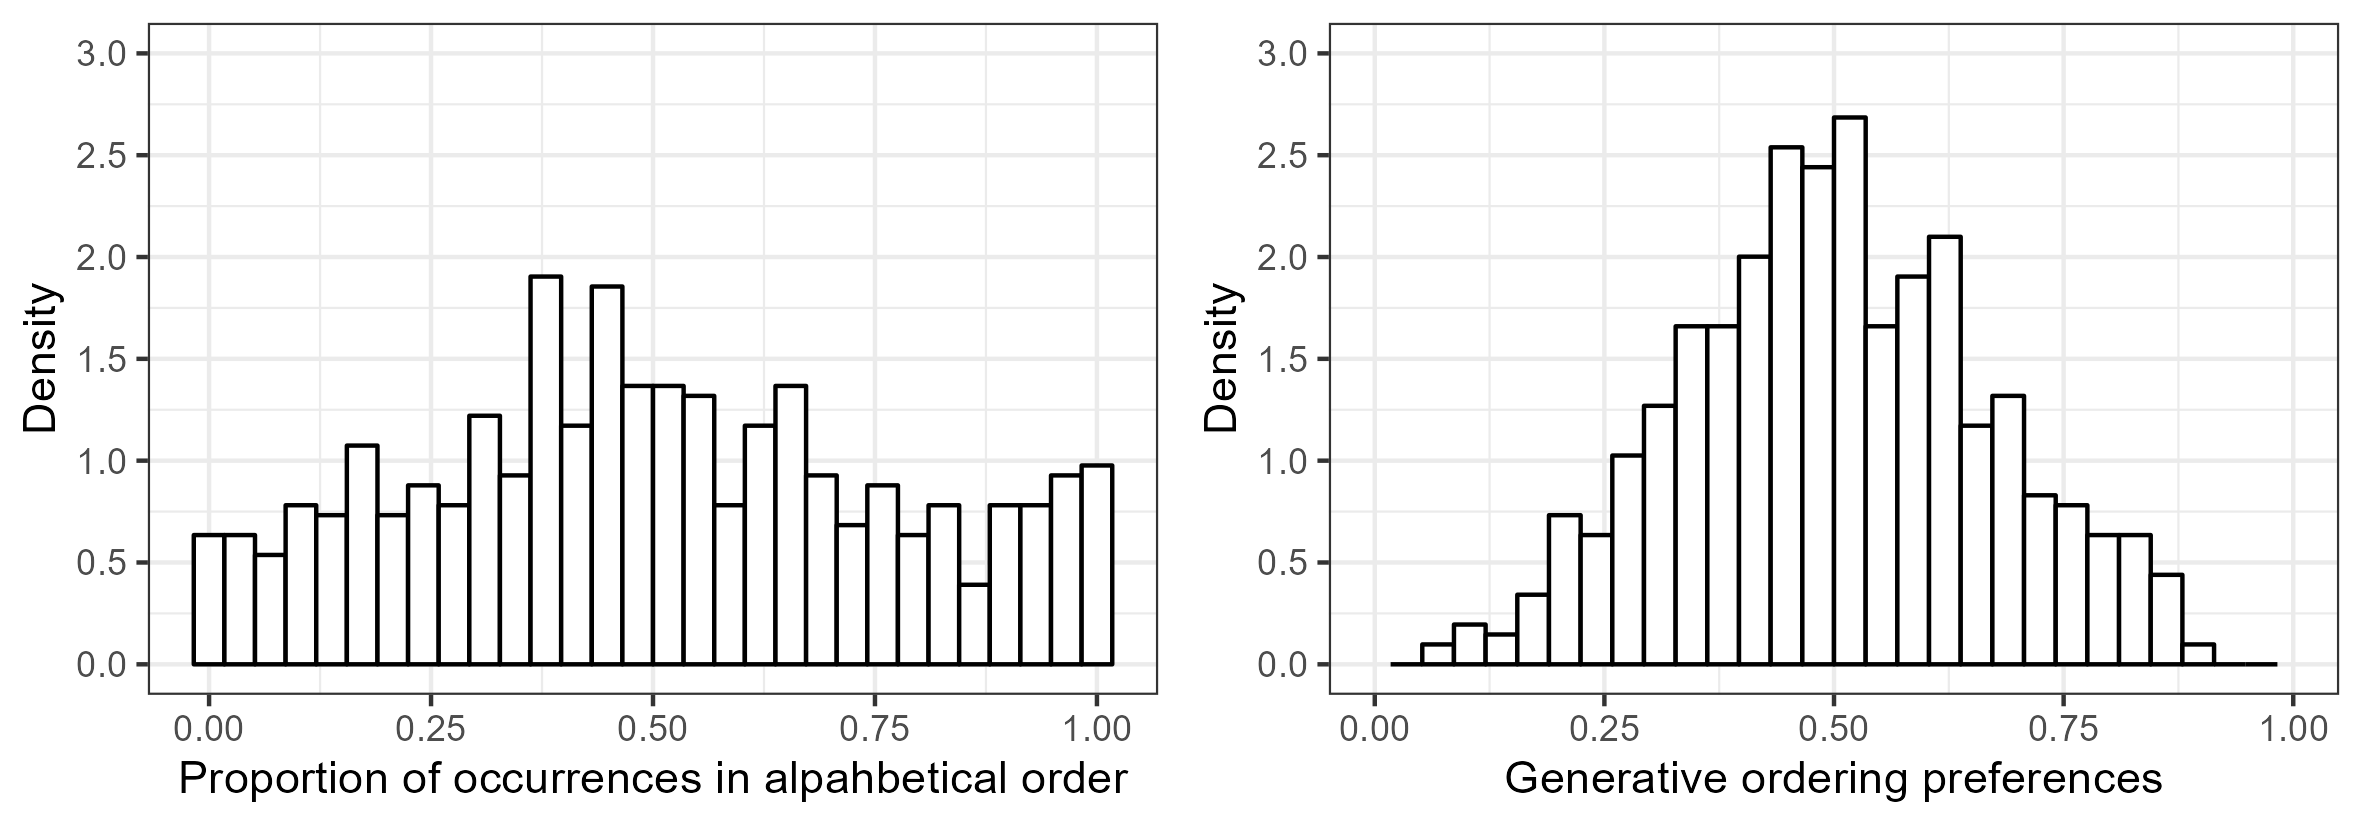
\includegraphics[width=1\linewidth]{Figures/corpus_plots} 

}

\caption[The left plot is a plot of the observed orderings of binomials in the corpus data from Morgan \& Levy (2015), the right is the plot of the generative preferences of binomials in the same corpus]{The left plot is a plot of the observed orderings of binomials in the corpus data from Morgan \& Levy (2015), the right is the plot of the generative preferences of binomials in the same corpus.}\label{fig:corpusplot1}
\end{figure}
\end{CodeChunk}

\hypertarget{model}{%
\section{Model}\label{model}}

Following Morgan \& Levy (2016b), we use a 2-alternative iterated
learning paradigm. In our iterated learning paradigm, at each
generation, learners hear N tokens of a given binomial with some in
alphabetical (AandB) and some in nonalphabetical (BandA) order. The
learner's goal is to learn the ordering preferences for each binomial.
After hearing all N tokens, the learner then produces N tokens to the
next generation. This process then repeats. Morgan \& Levy (2016b) used
a beta-binomial model: A learner has some prior over binomial ordering
preferences, which can be expressed as pseudocounts favoring each order
(e.g.~3 pseudocounts for AandB and 7 for BandA). Each time the learner
hears a binomial, they update their beliefs by adding 1 count to the
perceived order, e.g.~if they heard AandB, adding 1 AandB count. We
modify this by instead having the learner update their beliefs in
proportion to what they believe the intended order was: e.g.~if they
believe the intended utterance was AandB with 50\% probability and BandA
with 50\% probability, they will add 0.5 to each count. These updated
beliefs then influence their beliefs about future intended utterances
(Eq. \ref{eq:gibsonnoisy}).

Specifically, the prior probability over the binomial ordering
preferences, \(P(S_i)\), follows Equations \ref{eq:psi} and
\ref{eq:ptheta}. \(\alpha_1\) and \(\alpha_2\) are pseudocounts of the
alphabetical and nonalphabetical forms respectively.

\begin{equation}
\label{eq:psi}
S_i \sim Bernoulli(p_{theta})
\end{equation}

\begin{equation}
\label{eq:ptheta}
p_{theta} \sim Beta(\alpha_1, \alpha_2)
\end{equation}

After hearing a token, learners compute \(P(S_i = AandB|S_p)\) according
to Equation \ref{eq:gibsonnoisy}. \(P(S_i \to S_p)\) is determined by a
fixed noise parameter, which we will call \(p_{noise}\). \(p_{noise}\)
represents the learner's belief of how likely a binomial ordering is to
have been swapped (i.e., AandB being swapped to BandA or vice versa).

To initialize \(p_{theta}\), and thus \(P(S_i)\), before the learner
hears any data, we used the mean and concentration parametrization of
the beta distribution. The mean (\(\mu\)) represents the expectation of
the distribution (the mean value of draws from the distribution). The
concentration parameter (\(\nu\)) describes how dense the distribution
is. Before the learner hears any data, \(\mu\) is equal to the
generative preference for the binomial (taken from Morgan \& Levy,
2016b). \(\nu\) is a free parameter, set to 10 for all simulations in
this paper.\footnote{Changing \(\nu\) does not qualitatively change the
  pattern of the results for any simulations in the paper, as long as
  it's greater than 2.} \(\alpha_1\) and \(\alpha_2\) can also be
expressed in terms of \(\mu\) and \(\nu\):

\begin{equation}
\label{eq:alpha1}
\alpha_1 = \mu \cdot \nu
\end{equation}

\begin{equation}
\label{eq:alpha2}
\alpha_2 = (1-\mu) \cdot \nu
\end{equation}

For all future tokens, learners will use the updated \(P(S_i)\) from the
previous token, where \(P(S_i = AandB)\) is the expectation of
\(p_\theta\). Crucially, this value will be different for each token of
learning due to the update that occurs on the previous token.

\begin{equation}
\label{eq:expectationptheta}
P(S_i = AandB) = \mathbb{E}(p_\theta)
\end{equation}

We then use \(P(S_i)\) and \(p_{noise}\) to compute \(P(S_i|S_p)\),
following Equation \ref{eq:gibsonnoisy}. If the perceived binomial is
alphabetical (AandB), we compute the unnormalized probability of the
alphabetical and nonalphabetical orderings according to the below
equations. Note that the process is comparable if the perceived binomial
is nonalphabetical.

\begin{multline}
\label{eq:praw}
P_{raw}(S_i = AandB|S_p = AandB) \\ = P(S_i = AandB) \cdot (1 -  p_{noise})
\end{multline}

\begin{multline}
\label{eq:prawtwo}
P_{raw}(S_i = BandA|S_p = AandB) \\ = (1 - P(S_i = AandB)) \cdot p_{noise}
\end{multline}

After calculating the unnormalized (raw) probabilities, they are then
normalized:

\begin{myequation}%
\label{eq:phatalpha}
\hat{p}_{\alpha} = \frac{P_{raw}(S_i = AandB|S_p = AandB)}{P_{raw}(S_i = AandB | S_p = AandB) + P_{raw}(S_i = BandA|S_p = AandB)} %
\end{myequation}

\begin{equation}
\label{eq:phatnotalpha}
\hat{p}_{\neg\alpha} = 1 - \hat{p}_\alpha
\end{equation}

\noindent where \(\hat{p}_\alpha\) is the probability that the intended
binomial order was the alphabetical order, and \(\hat{p}_{\neg\alpha}\)
is the probability that the intended binomial order was the
nonalphabetical order.

We then update \(\alpha_1'\) and \(\alpha_2'\) to be used as the
parameters of \(p_\theta\), and thus \(P(S_i)\), when the learner hears
the next token. This update is done according to the following equation:

\begin{equation}
\label{eq:alpha1prime}
\alpha_1' = \alpha_1 + \hat{p}_\alpha
\end{equation}

\begin{equation}
\label{eq:alpha2prime}
\alpha_2' = \alpha_2 + \hat{p}_{\neg\alpha}
\end{equation}

Note that when the learner hears any binomial, they update their beliefs
about the probability of both the alphabetical \emph{and}
nonalphabetical forms of the binomial (in proportion to how likely they
believe each ordering was intended by the speaker).

When the learner is done hearing N tokens and updating their beliefs of
\(P(S_i)\) for a given binomial, they then produce N tokens for the next
generation of learners. These are generated binomially, where
\(\theta = \mathbb{E}(p_\theta)\) is the inferred probability of the
alphabetical form of a given binomial. For the first generation of
speakers (before any learning has occurred), \(\theta\) is initialized
at 0.5.

When producing each token, there is also a possibility that the speaker
makes an error and produces an unintended ordering of the binomial. The
speaker error is analogous to a speaker choosing to produce a binomial
ordering (AandB or BandA), and then accidentally flipping it. For
example, perhaps they intended to say \emph{butter and bread}, but
accidentally said \emph{bread and butter} (or vice versa). Note that the
``unintended ordering'' is whichever order the speaker did not choose to
produce on that trial, regardless of the overall preference for the
binomial. In order to model this, the speaker produces a token in the
unintended order with probability \(p_{SpeakerNoise}\). This is a fixed
parameter in the model and remains constant across binomials and
generations.

This process continues iteratively for \(ngen\) generations.

\hypertarget{results}{%
\section{Results}\label{results}}

We present our results in two main sections. The first section
demonstrates the effects of the speaker and listener noise parameters
(\(p_{noise}\) and \(p_{SpeakerNoise}\) respectively) on simulations of
individual binomials. The aim of this section is to examine whether the
model can account for frequency-dependent preference extremity across
individual binomials varying in frequency.

The second section compares our model's predicted binomial orderings
across a range of binomials to the real-world corpus-wide distribution.
In this section, rather than simulating individual binomials, we
simulate the distribution of binomial orderings across the entire
dataset of binomials from Morgan \& Levy (2015) with the intent of
examining whether our model can capture the corpus-wide distribution.

\hypertarget{speaker-vs-listener-noise}{%
\subsection{Speaker vs Listener Noise}\label{speaker-vs-listener-noise}}

First we demonstrate that frequency-dependent preference extremity does
not arise when there is no listener or speaker noise.\footnote{All code
  and results can be found publicly available here:
  \url{https://github.com/znhoughton/Noisy-Channel-Iterated-Learning}}
Instead we see convergence to the prior, which is expected following
Griffiths \& Kalish (2007). They demonstrated that when learners sample
from the posterior in an iterated learning paradigm, the stationary
distribution converges to the prior. To confirm this, we simulated the
evolution of a single binomial across 500 generations with various N
(50, 100, 500, 1000, and 10,000). The generative preference was 0.6.
1000 chains were run. We then examined the model's inferred ordering
preference in the final generation. A visualization of the results is
presented in Figure \ref{fig:noNoisePlot}.

\begin{CodeChunk}
\begin{figure}[tb]

{\centering 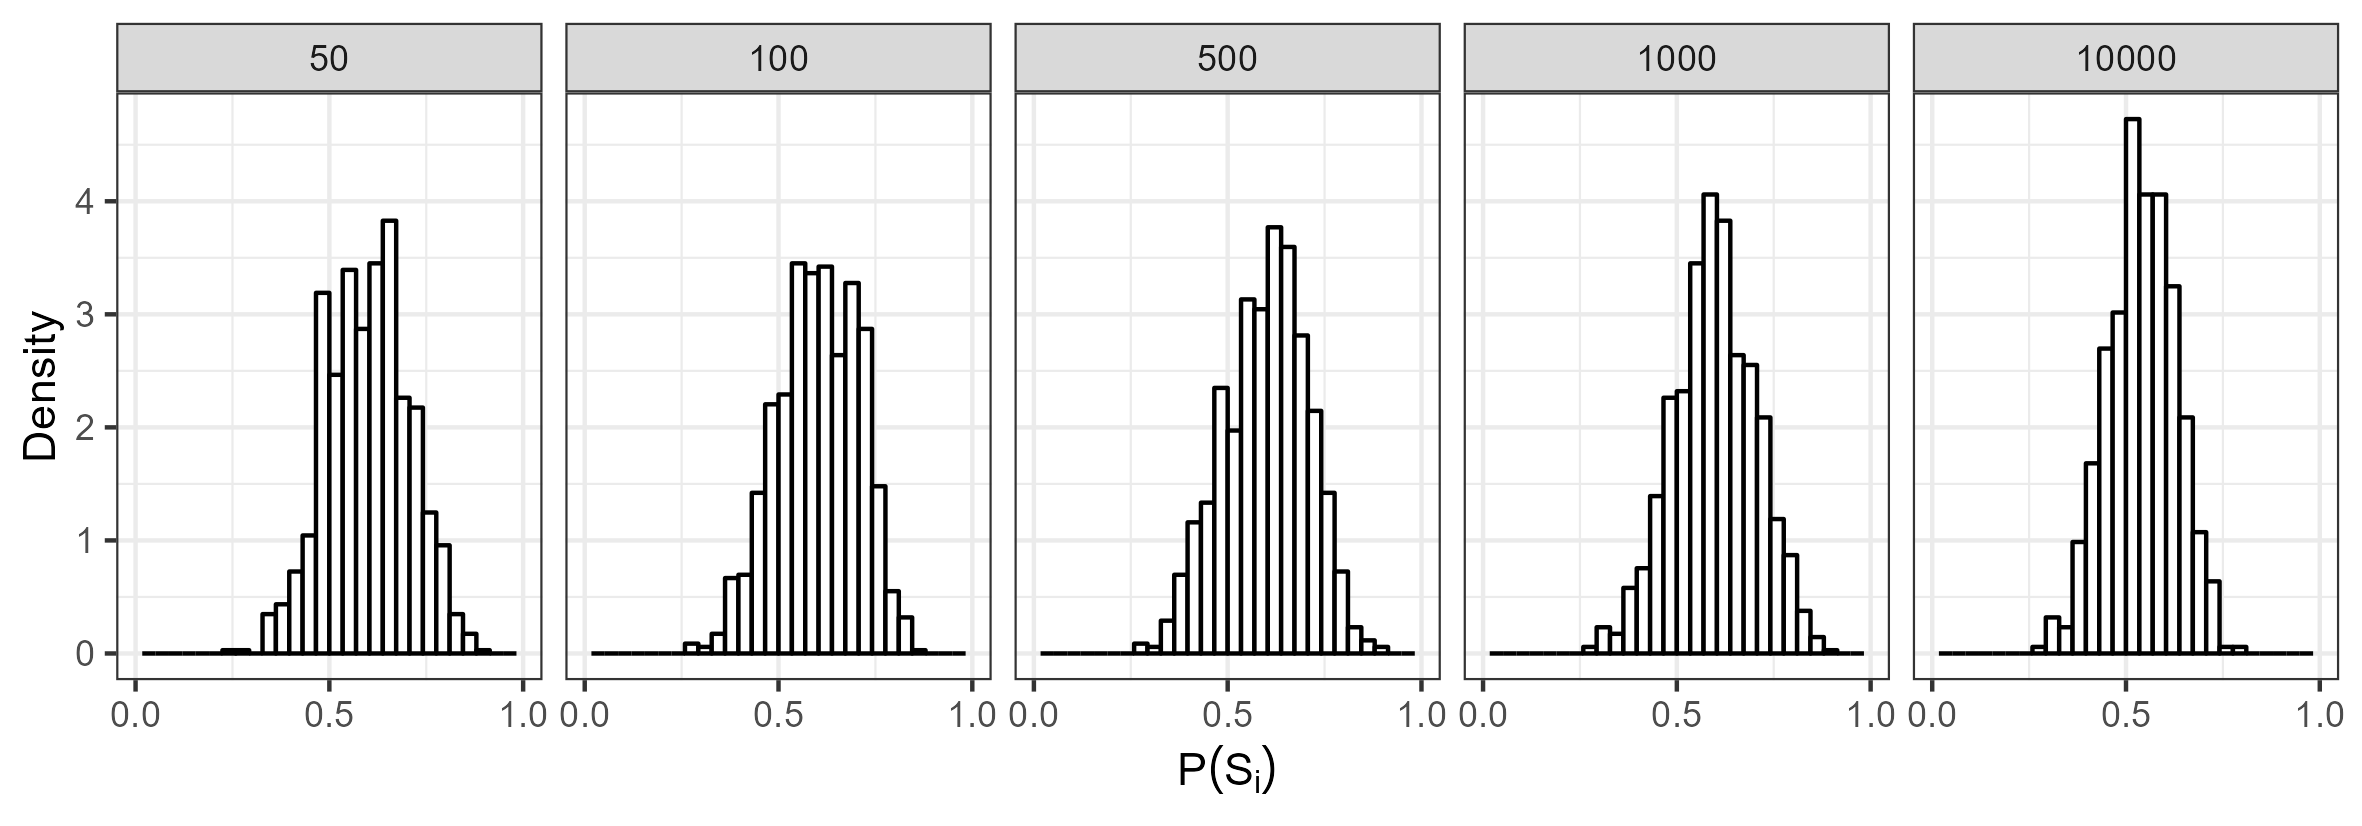
\includegraphics[width=1\linewidth]{Figures/noNoise} 

}

\caption[A plot of the distribution of simulated binomials at the 500th generation, varying in frequency]{A plot of the distribution of simulated binomials at the 500th generation, varying in frequency. The top value represents N, which is the overall frequency of a binomial regardless of ordering (i.e., count(AandB) + count(BandA)). On the x-axis is the predicted probability of producing the binomial in alphabetical form. On the y-axis is probability density. Speaker and listener noise was set to 0. The generative preference was 0.6, and nu was set to 10. 1000 chains were run. Note that all values of N produce dense distributions clustered around 0.6 (i.e., there is no frequency-dependent preference extremity).}\label{fig:noNoisePlot}
\end{figure}
\end{CodeChunk}

We then systematically manipulated N, listener noise (\(p_{noise}\)) and
speaker noise (\(p_{SpeakerNoise}\)). Specifically, we varied N across
100, 1000, and 10000, and listener and speaker noise were varied across
0, 0.033, 0.066, and 0.1. We ran simulations for every combination of
these values (Figure \ref{fig:fullsimsplot}. For these simulations, the
generative preference was set to 0.6 and 1000 chains were run across 500
generations.

Our results suggest that frequency-dependent preference extremity does
arise from the model when noise is introduced, but only if listener
noise is greater than speaker noise. Further our results demonstrate
that if listener noise is greater than speaker noise, then the greater
the difference between the listener and speaker noise, the stronger the
preference extremity effect (this is demonstrated by moving vertically
down the column labeled \(p_{SpeakerNoise} = 0\) in Figure
\ref{fig:fullsimsplot}).

Interestingly this preference extremity disappears if the listener's
noise parameter is less than or equal to the speaker's noise parameter.
For example, notice how if you split the plot along the diagonal, all
the plots on the top half, including the diagonal, show no evidence of
preference extremity. These graphs are all visualizations where the
speaker noise is greater than the listener noise.

\begin{CodeChunk}
\begin{figure*}[!htb]
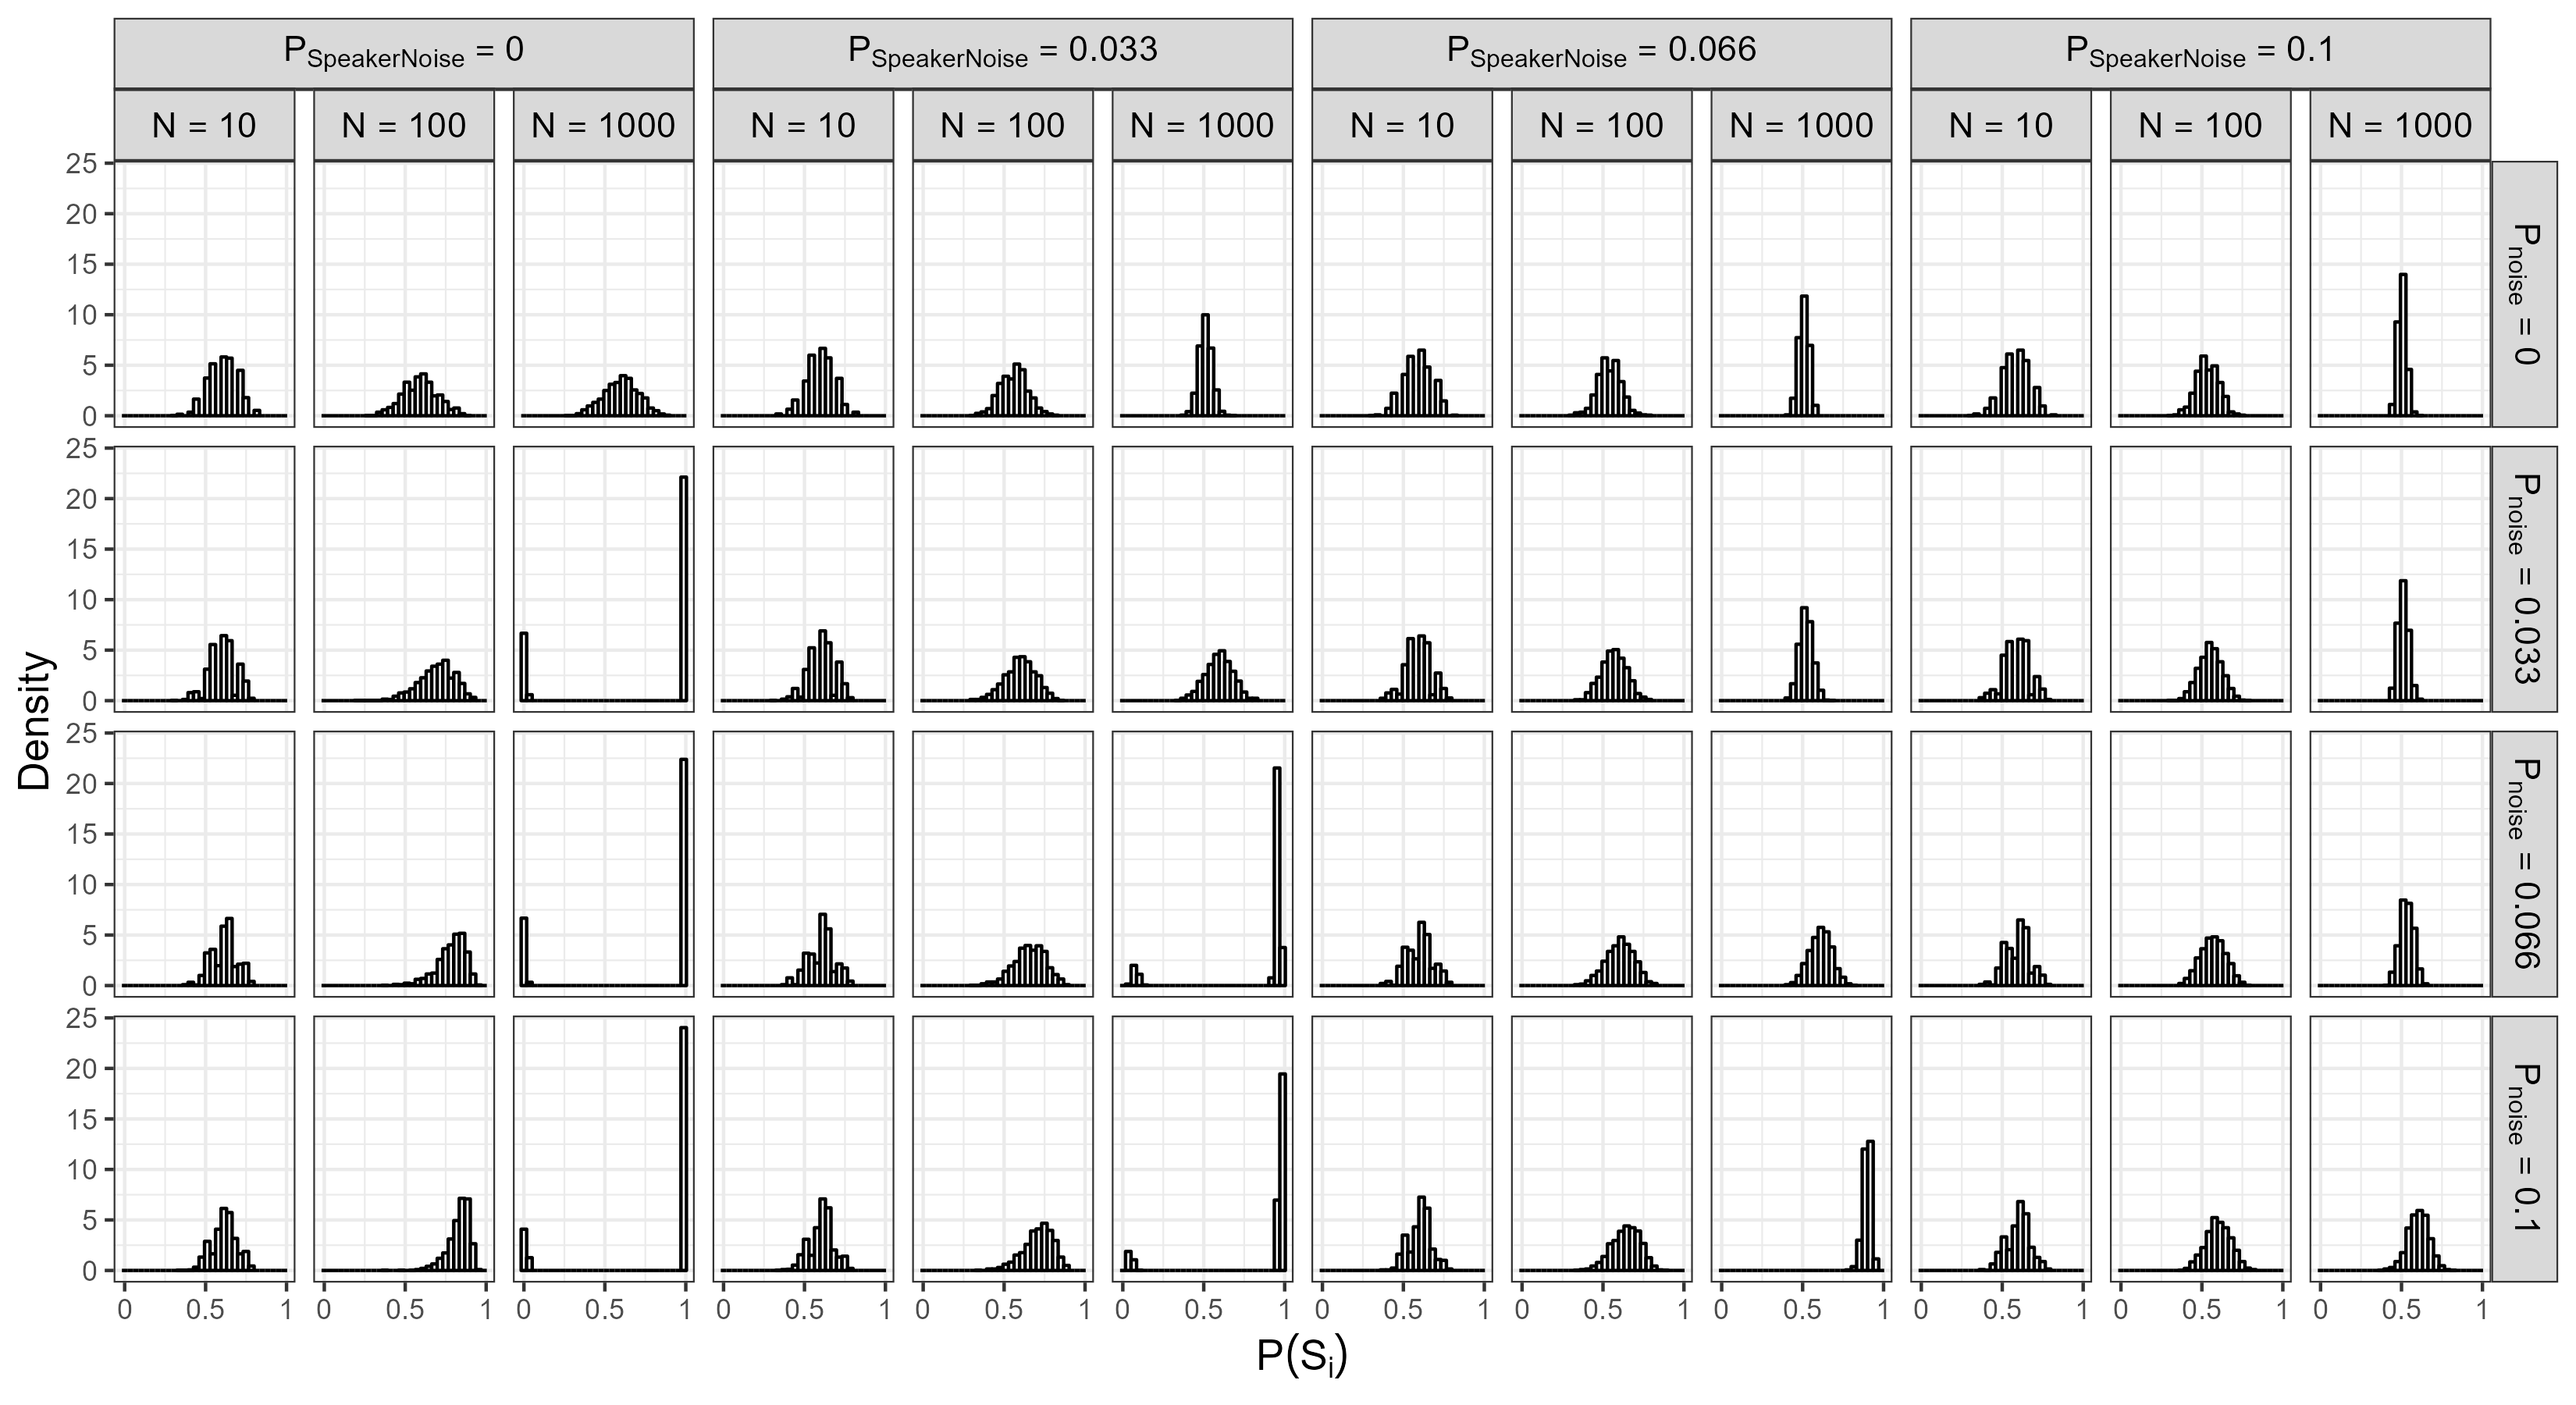
\includegraphics[width=1\linewidth]{Figures/full_plot_smallerN} \caption[Our simulation results for every combination of speaker noise, listener noise, and N]{Our simulation results for every combination of speaker noise, listener noise, and N. Note that there is an increase in ordering preference extrmity as N increases when listener noise is greater than speaker noise. N corresponds to the overall frequency of the binomial (count of AandB plus count of BandA) and varies across 10, 100, and 1000. Both speaker and listener noise were varied across 0, 0.033, 0.066, and 0.1. The distributions in the plot demonstrate the inferred ordering preference at the 500th generation.}\label{fig:fullsimsplot}
\end{figure*}
\end{CodeChunk}

It is useful to revisit here what the speaker and listener noise
parameters represent. The speaker noise parameter is how often the
speaker produces an error and the listener noise parameter is the
listeners' belief of how noisy the environment is. Note that a speaker
error here is not whether the speaker produces the more frequent
binomial ordering, but rather whether the speaker produces the intended
binomial ordering. In other words, if a speaker intends to produce
\emph{butter and bread}, and instead produces \emph{bread and butter},
this is an error in our model. Framed this way, one explanation for our
results is that when the listener is inferring more noise than the
speakers are producing, they are relying more on their inferences, which
can become more and more extreme. On the other hand, if they're not
inferring enough noise, then they will rely more on the data. The
greater the speaker noise, due to how we operationalized speaker noise,
the more balanced the data will be.

Thus our model makes a novel prediction: In order to account for
frequency-dependent preference extremity, listeners must be inferring
more noise than speakers are actually producing.

\hypertarget{corpus-data}{%
\subsection{Corpus Data}\label{corpus-data}}

Finally, we now demonstrate that our model also predicts the
language-wide distribution of binomial preference strengths seen in the
corpus data. In order to demonstrate this, we simulated model
predictions for all 594 binomials from Morgan \& Levy (2015). The model
estimated the ordering preference across 500 generations with 10 chains
each. Values for the generative preference and N for each binomial were
taken from (Morgan \& Levy, 2015)'s corpus. Listener noise was set to
0.02 and speaker noise to 0.005. Note that we scale N based on an
estimated lifetime exposure of 300 million tokens (Levy et al., 2012).

Our results demonstrate that our model can approximate the distribution
in the corpus data (See Figure \ref{fig:corpusourmodel}). In other
words, the corpus-wide distribution of binomial orderings according to
our model is similar to the ordering we see in actual corpus data.
Further, the distribution is qualitatively similar regardless of
listener and speaker noise parameters, as long as listener noise is
greater than speaker noise. Altogether, this suggests that our model
both captures the phenomenon of frequency-dependent preference
extremity, but also in capturing it our model also predicts a similar
distribution of binomial orderings to what we see in corpus data.

\begin{CodeChunk}
\begin{figure}[!htb]

{\centering 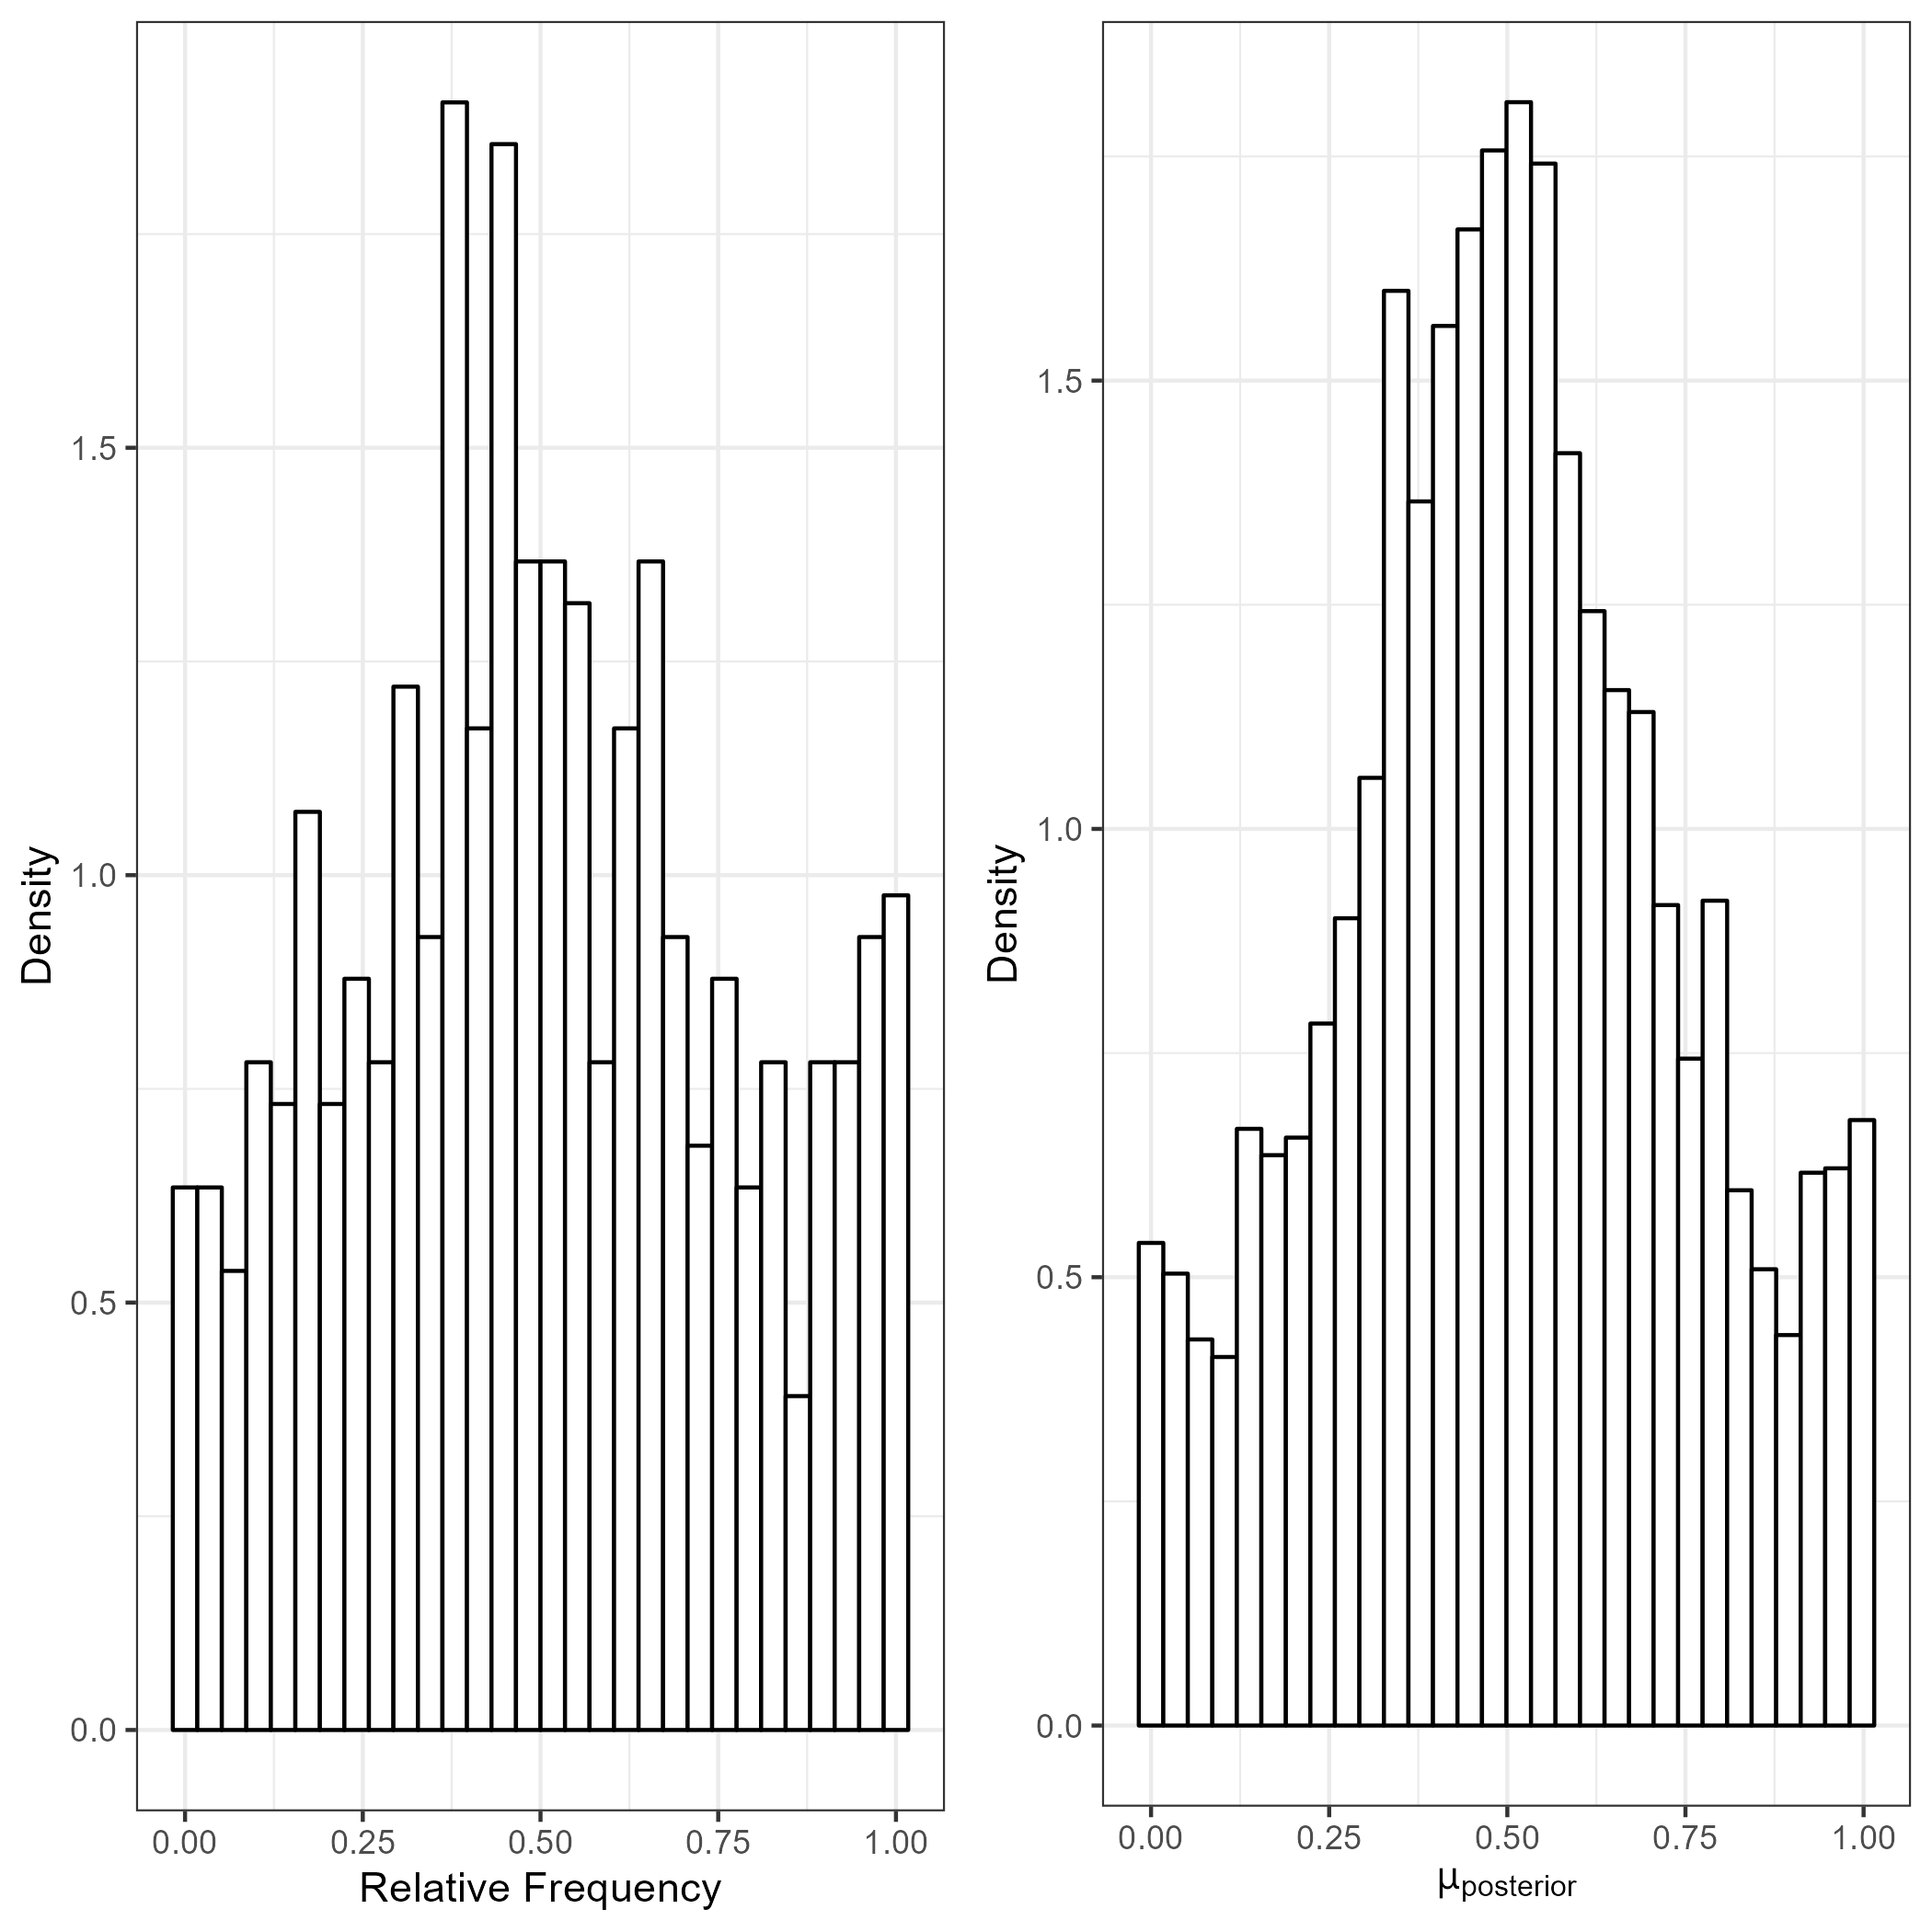
\includegraphics[width=1\linewidth]{Figures/corpus_plot_and_ours} 

}

\caption[A plot of the stationary distribution of ordering preferences in the corpus data from Morgan \& Levy (2015) and the distribution of ordering preferences after 500 generations of our iterated learning model (left and right respectively)]{A plot of the stationary distribution of ordering preferences in the corpus data from Morgan \& Levy (2015) and the distribution of ordering preferences after 500 generations of our iterated learning model (left and right respectively). For our simulations, the binomial frequencies and generative preferences were matched with the corpus data. Listener noise was set to 0.02, and speaker noise was set to 0.005.}\label{fig:corpusourmodel}
\end{figure}
\end{CodeChunk}

\hypertarget{conclusion}{%
\section{Conclusion}\label{conclusion}}

The present study examined whether a noisy-channel processing model
(Gibson et al., 2013) integrated in an iterated learning model (Morgan
\& Levy, 2016b) can capture the effects of frequency-dependent
preference extremity. Our results demonstrate that frequency-dependent
preference extremity can emerge from a noisy-channel processing model
when listeners infer more noise in the environment than the speakers
actually produce. Our results also make novel predictions. For example,
if our current model is accurate, it suggests that listeners assume more
noise than the speakers produce. Further, it suggests that for
high-frequency binomials, such as \emph{butter and bread}, hearing
\emph{butter and bread} may activate \emph{bread and butter} more
strongly than \emph{butter and bread}. Finally, it seems more unlikely
that a speaker would unintentionally produce the unintended ordering for
high-frequency binomials than low-frequency binomials (e.g., producing
\emph{butter and bread,} when they mean to say \emph{bread and butter)}.
Thus it will also be interesting to examine models that don't use a
fixed speaker-noise parameter.

\hypertarget{acknowledgements}{%
\section{Acknowledgements}\label{acknowledgements}}

This research was supported by the UC Davis Society of Hellman Fellows
Program and the UC Davis College of Letters and Science.

\hypertarget{references}{%
\section{References}\label{references}}

\setlength{\parindent}{-0.1in} 
\setlength{\leftskip}{0.125in}

\noindent

\hypertarget{refs}{}
\begin{CSLReferences}{1}{0}
\leavevmode\vadjust pre{\hypertarget{ref-feltyMisperceptionsSpokenWords}{}}%
Albert Felty, R., Buchwald, A., Gruenenfelder, T. M., \& Pisoni, D. B.
(2013). Misperceptions of spoken words: Data from a random sample of
american english words. \emph{The Journal of the Acoustical Society of
America}, \emph{134}(1), 572--585.

\leavevmode\vadjust pre{\hypertarget{ref-benor2006}{}}%
Benor, S. B., \& Levy, R. (2006). The chicken or the egg? A
probabilistic analysis of english binomials. \emph{Language}, 233278.

\leavevmode\vadjust pre{\hypertarget{ref-christiansonThematicRolesAssigned2001}{}}%
Christianson, K., Hollingworth, A., Halliwell, J. F., \& Ferreira, F.
(2001). Thematic roles assigned along the garden path linger.
\emph{Cognitive Psychology}, \emph{42}(4), 368--407.
\url{https://doi.org/10.1006/cogp.2001.0752}

\leavevmode\vadjust pre{\hypertarget{ref-ferdinandCognitiveRootsRegularization2019}{}}%
Ferdinand, V., Kirby, S., \& Smith, K. (2019). The cognitive roots of
regularization in language. \emph{Cognition}, \emph{184}, 53--68.
\url{https://doi.org/10.1016/j.cognition.2018.12.002}

\leavevmode\vadjust pre{\hypertarget{ref-ferreiraGoodEnoughApproach2007}{}}%
Ferreira, F., \& Patson, N. D. (2007). The {`}Good Enough{'} Approach to
Language Comprehension. \emph{Language and Linguistics Compass},
\emph{1}(1-2), 71--83.
\url{https://doi.org/10.1111/j.1749-818X.2007.00007.x}

\leavevmode\vadjust pre{\hypertarget{ref-ganongPhoneticCategorizationAuditory1980}{}}%
Ganong, W. F. (1980). Phonetic categorization in auditory word
perception. \emph{Journal of Experimental Psychology: Human Perception
and Performance}, \emph{6}(1), 110.
\url{https://psycnet.apa.org/record/1981-07020-001}

\leavevmode\vadjust pre{\hypertarget{ref-gibsonNoisy2013}{}}%
Gibson, E., Bergen, L., \& Piantadosi, S. T. (2013). Rational
integration of noisy evidence and prior semantic expectations in
sentence interpretation. \emph{Proceedings of the National Academy of
Sciences}, \emph{110}(20), 8051--8056.
\url{https://doi.org/10.1073/pnas.1216438110}

\leavevmode\vadjust pre{\hypertarget{ref-griffithsLanguageEvolutionIterated2007}{}}%
Griffiths, T. L., \& Kalish, M. L. (2007). Language evolution by
iterated learning with bayesian agents. \emph{Cognitive Science},
\emph{31}(3), 441--480. \url{https://doi.org/10.1080/15326900701326576}

\leavevmode\vadjust pre{\hypertarget{ref-harmonPuttingOldTools2017}{}}%
Harmon, Z., \& Kapatsinski, V. (2017). Putting old tools to novel uses:
The role of form accessibility in semantic extension. \emph{Cognitive
Psychology}, \emph{98}, 22--44.
\url{https://doi.org/10.1016/j.cogpsych.2017.08.002}

\leavevmode\vadjust pre{\hypertarget{ref-hudsonkamGettingItRight2009}{}}%
Hudson Kam, C. L., \& Newport, E. L. (2009). Getting it right by getting
it wrong: When learners change languages. \emph{Cognitive Psychology},
\emph{59}(1), 30--66.
\url{https://doi.org/10.1016/j.cogpsych.2009.01.001}

\leavevmode\vadjust pre{\hypertarget{ref-kapatsinskiChangingMindsChanging2018}{}}%
Kapatsinski, V. (2018). \emph{Changing minds changing tools: From
learning theory to language acquisition to language change}. MIT Press.
\url{https://books.google.com/books?hl=en\&lr=\&id=YZxjDwAAQBAJ\&oi=fnd\&pg=PR5\&dq=kapatsinski+changing+minds\&ots=9bGhgkCaY0\&sig=MHfWF9cbhbtMmx33a0FYSM6AMAs}

\leavevmode\vadjust pre{\hypertarget{ref-keshevNoisyBetterRare2021}{}}%
Keshev, M., \& Meltzer-Asscher, A. (2021). Noisy is better than rare:
Comprehenders compromise subject-verb agreement to form more probable
linguistic structures. \emph{Cognitive Psychology}, \emph{124}, 101359.
\url{https://doi.org/10.1016/j.cogpsych.2020.101359}

\leavevmode\vadjust pre{\hypertarget{ref-kirbyCumulativeCulturalEvolution2008}{}}%
Kirby, S., Cornish, H., \& Smith, K. (2008). Cumulative cultural
evolution in the laboratory: An experimental approach to the origins of
structure in human language. \emph{Proceedings of the National Academy
of Sciences}, \emph{105}(31), 10681--10686.
\url{https://doi.org/10.1073/pnas.0707835105}

\leavevmode\vadjust pre{\hypertarget{ref-levyNoisychannel2008}{}}%
Levy, R. (2008). \emph{A noisy-channel model of human sentence
comprehension under uncertain input}. 234243.
\url{https://aclanthology.org/D08-1025.pdf}

\leavevmode\vadjust pre{\hypertarget{ref-levyProcessingExtraposedStructures2012}{}}%
Levy, R., Fedorenko, E., Breen, M., \& Gibson, E. (2012). The processing
of extraposed structures in english. \emph{Cognition}, \emph{122}(1),
12--36. \url{https://doi.org/10.1016/j.cognition.2011.07.012}

\leavevmode\vadjust pre{\hypertarget{ref-linSyntacticAnnotationsGoogle2012}{}}%
Lin, Y., Michel, J.-B., Lieberman, E. A., Orwant, J., Brockman, W., \&
Petrov, S. (2012). \emph{Syntactic annotations for the google books
ngram corpus}. 169174. \url{https://aclanthology.org/P12-3029.pdf}

\leavevmode\vadjust pre{\hypertarget{ref-liu2020}{}}%
Liu, Z., \& Morgan, E. (2020). \emph{Frequency-dependent regularization
in constituent ordering preferences.}
\url{https://www.cognitivesciencesociety.org/cogsci20/papers/0751/0751.pdf}

\leavevmode\vadjust pre{\hypertarget{ref-liu2021}{}}%
Liu, Z., \& Morgan, E. (2021). \emph{Frequency-dependent regularization
in syntactic constructions}. 387389.
\url{https://aclanthology.org/2021.scil-1.41.pdf}

\leavevmode\vadjust pre{\hypertarget{ref-morganModelingIdiosyncraticPreferences2015}{}}%
Morgan, E., \& Levy, R. (2015). \emph{Modeling idiosyncratic preferences
: How generative knowledge and expression frequency jointly determine
language structure}. 1649--1654.

\leavevmode\vadjust pre{\hypertarget{ref-morgan2016}{}}%
Morgan, E., \& Levy, R. (2016a). Abstract knowledge versus direct
experience in processing of binomial expressions. \emph{Cognition},
\emph{157}, 384--402.
\url{https://doi.org/10.1016/j.cognition.2016.09.011}

\leavevmode\vadjust pre{\hypertarget{ref-morganFrequencydependentRegularizationIterated2016}{}}%
Morgan, E., \& Levy, R. (2016b). Frequency-dependent regularization in
iterated learning. \emph{The Evolution of Language: Proceedings of the
11th International Conference}.

\leavevmode\vadjust pre{\hypertarget{ref-poppelsStructuresensitiveNoiseInference2016}{}}%
Poppels, T., \& Levy, R. (2016). \emph{Structure-sensitive noise
inference: Comprehenders expect exchange errors.}
\url{https://tpoppels.github.io/files/2016-poppels-levy-cogsci-proceedings.pdf}

\leavevmode\vadjust pre{\hypertarget{ref-realiEvolutionFrequencyDistributions2009}{}}%
Reali, F., \& Griffiths, T. L. (2009). The evolution of frequency
distributions: Relating regularization to inductive biases through
iterated learning. \emph{Cognition}, \emph{111}(3), 317--328.
\url{https://doi.org/10.1016/j.cognition.2009.02.012}

\leavevmode\vadjust pre{\hypertarget{ref-robenaltJudgmentEvidenceStatistical2015}{}}%
Robenalt, C., \& Goldberg, A. E. (2015). Judgment evidence for
statistical preemption: It is relatively better to vanish than to
disappear a rabbit, but a lifeguard can equally well backstroke or swim
children to shore. \emph{Cognitive Linguistics}, \emph{26}(3), 467--503.
\url{https://doi.org/10.1515/cog-2015-0004}

\leavevmode\vadjust pre{\hypertarget{ref-saffranStatisticalLearning8MonthOld1996}{}}%
Saffran, J. R., Aslin, R. N., \& Newport, E. L. (1996). Statistical
Learning by 8-Month-Old Infants. \emph{Science}, \emph{274}(5294),
1926--1928. \url{https://doi.org/10.1126/science.274.5294.1926}

\leavevmode\vadjust pre{\hypertarget{ref-schneiderNoisyChannelModel2020}{}}%
Schneider, J., Perkins, L., \& Feldman, N. H. (2020). \emph{A noisy
channel model for systematizing unpredictable input variation}. 533547.
\url{http://www.lingref.com/bucld/44/BUCLD44-43.pdf}

\leavevmode\vadjust pre{\hypertarget{ref-singletonWhenLearnersSurpass2004}{}}%
Singleton, J. L., \& Newport, E. L. (2004). When learners surpass their
models: The acquisition of american sign language from inconsistent
input. \emph{Cognitive Psychology}, \emph{49}(4), 370407.
\url{https://www.sciencedirect.com/science/article/pii/S0010028504000295}

\leavevmode\vadjust pre{\hypertarget{ref-theakstonRoleEntrenchmentChildren2004}{}}%
Theakston, A. L. (2004). The role of entrenchment in children{'}s and
adults{'} performance on grammaticality judgment tasks. \emph{Cognitive
Development}, \emph{19}(1), 15--34.
\url{https://doi.org/10.1016/j.cogdev.2003.08.001}

\leavevmode\vadjust pre{\hypertarget{ref-yuRapidWordLearning2007}{}}%
Yu, C., \& Smith, L. B. (2007). Rapid Word Learning Under Uncertainty
via Cross-Situational Statistics. \emph{Psychological Science},
\emph{18}(5), 414--420.
\url{https://doi.org/10.1111/j.1467-9280.2007.01915.x}

\end{CSLReferences}

\bibliographystyle{apacite}


\end{document}
